%%%%%%%%%%%%%%%%%%%%%%%%%%%%%%%%%%%%%%%%%%%%%%%%%%%%%%%%%%%%%%%%%%%%%%%%%%%
%% This file is part of the book
%%
%% Algorithmic Graph Theory
%% http://code.google.com/p/graph-theory-algorithms-book/
%%
%% Copyright (C) 2009, 2010, 2011 Minh Van Nguyen <nguyenminh2@gmail.com>
%%
%% See the file COPYING for copying conditions.
%%%%%%%%%%%%%%%%%%%%%%%%%%%%%%%%%%%%%%%%%%%%%%%%%%%%%%%%%%%%%%%%%%%%%%%%%%%

\subfigure[Original undirected graph.]{
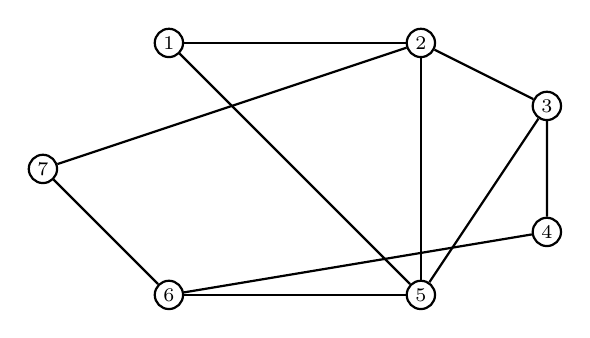
\begin{tikzpicture}
[lineDecorate/.style={-,thick},%
  nodeDecorate/.style={shape=circle,inner sep=1.5pt,draw,thick},%
  scale=0.8]
%% nodes or vertices
\foreach \nodename/\x/\y in {2/4/4, 1/0/4, 3/6/3, 4/6/1, 5/4/0, 7/-2/2, 6/0/0}
{
  \node (\nodename) at (\x,\y) [nodeDecorate] {\scriptsize$\nodename$};
}
%% edges or lines
\path
\foreach \startnode/\endnode in {
  1/2, 1/5, 2/3, 2/5, 2/7, 3/4, 3/5, 4/6, 5/6, 6/7}
{
  (\startnode) edge[lineDecorate] node {} (\endnode)
};
\end{tikzpicture}
}
%%
%%
\qquad
\subfigure[First iteration of while loop.]{
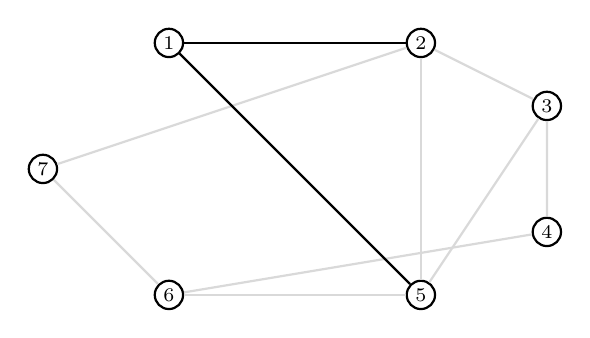
\begin{tikzpicture}
[darkLine/.style={-,thick},%
  lightLine/.style={-,thick,color=gray!30},%
  nodeDecorate/.style={shape=circle,inner sep=1.5pt,draw,thick},%
  scale=0.8]
%% nodes or vertices
\foreach \nodename/\x/\y in {2/4/4, 1/0/4, 3/6/3, 4/6/1, 5/4/0, 7/-2/2, 6/0/0}
{
  \node (\nodename) at (\x,\y) [nodeDecorate] {\scriptsize$\nodename$};
}
%% light edges or lines
\path
\foreach \startnode/\endnode in {2/3, 2/5, 2/7, 3/4, 3/5, 4/6, 5/6, 6/7}
{
  (\startnode) edge[lightLine] node {} (\endnode)
};
%% dark edges or lines
\path
\foreach \startnode/\endnode in {1/2, 1/5}
{
  (\startnode) edge[darkLine] node {} (\endnode)
};
\end{tikzpicture}
}
%%
%%
\subfigure[Second iteration of while loop.]{
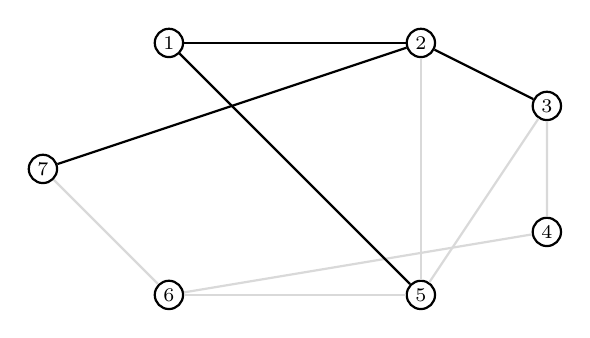
\begin{tikzpicture}
[darkLine/.style={-,thick},%
  lightLine/.style={-,thick,color=gray!30},%
  nodeDecorate/.style={shape=circle,inner sep=1.5pt,draw,thick},%
  scale=0.8]
%% nodes or vertices
\foreach \nodename/\x/\y in {2/4/4, 1/0/4, 3/6/3, 4/6/1, 5/4/0, 7/-2/2, 6/0/0}
{
  \node (\nodename) at (\x,\y) [nodeDecorate] {\scriptsize$\nodename$};
}
%% light edges or lines
\path
\foreach \startnode/\endnode in {2/5, 3/4, 3/5, 4/6, 5/6, 6/7}
{
  (\startnode) edge[lightLine] node {} (\endnode)
};
%% dark edges or lines
\path
\foreach \startnode/\endnode in {1/2, 1/5, 2/3, 2/7}
{
  (\startnode) edge[darkLine] node {} (\endnode)
};
\end{tikzpicture}
}
%%
%%
\qquad
\subfigure[Third iteration of while loop.]{
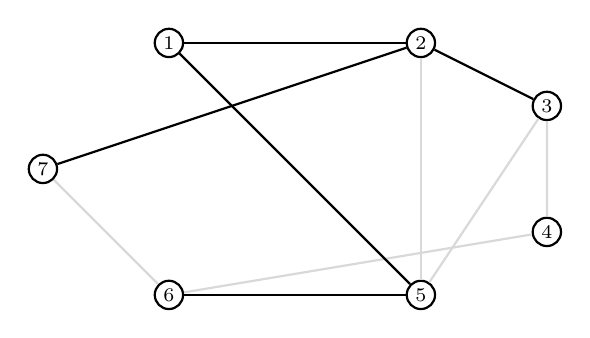
\begin{tikzpicture}
[darkLine/.style={-,thick},%
  lightLine/.style={-,thick,color=gray!30},%
  nodeDecorate/.style={shape=circle,inner sep=1.5pt,draw,thick},%
  scale=0.8]
%% nodes or vertices
\foreach \nodename/\x/\y in {2/4/4, 1/0/4, 3/6/3, 4/6/1, 5/4/0, 7/-2/2, 6/0/0}
{
  \node (\nodename) at (\x,\y) [nodeDecorate] {\scriptsize$\nodename$};
}
%% light edges or lines
\path
\foreach \startnode/\endnode in {2/5, 3/4, 3/5, 4/6, 6/7}
{
  (\startnode) edge[lightLine] node {} (\endnode)
};
%% dark edges or lines
\path
\foreach \startnode/\endnode in {1/2, 1/5, 2/3, 2/7, 5/6}
{
  (\startnode) edge[darkLine] node {} (\endnode)
};
\end{tikzpicture}
}
%%
%%
\subfigure[Fourth iteration of while loop.]{
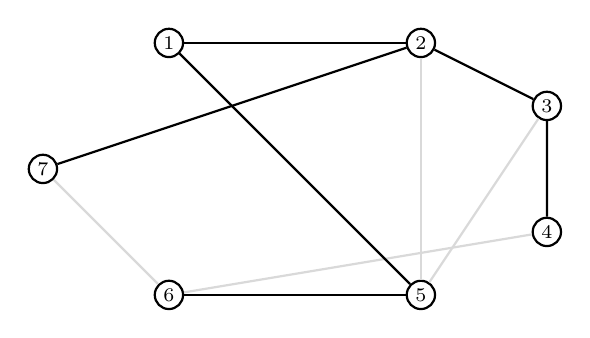
\begin{tikzpicture}
[darkLine/.style={-,thick},%
  lightLine/.style={-,thick,color=gray!30},%
  nodeDecorate/.style={shape=circle,inner sep=1.5pt,draw,thick},%
  scale=0.8]
%% nodes or vertices
\foreach \nodename/\x/\y in {2/4/4, 1/0/4, 3/6/3, 4/6/1, 5/4/0, 7/-2/2, 6/0/0}
{
  \node (\nodename) at (\x,\y) [nodeDecorate] {\scriptsize$\nodename$};
}
%% light edges or lines
\path
\foreach \startnode/\endnode in {2/5, 3/5, 4/6, 6/7}
{
  (\startnode) edge[lightLine] node {} (\endnode)
};
%% dark edges or lines
\path
\foreach \startnode/\endnode in {1/2, 1/5, 2/3, 2/7, 3/4, 5/6}
{
  (\startnode) edge[darkLine] node {} (\endnode)
};
\end{tikzpicture}
}
%%
%%
\qquad
\subfigure[Final BFS tree.]{
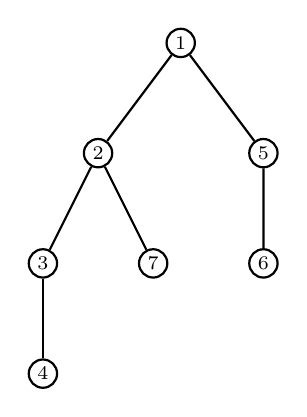
\begin{tikzpicture}
[lineDecorate/.style={-,thick},%
  nodeDecorate/.style={shape=circle,inner sep=1.5pt,draw,thick},%
  scale=1.4]
%% nodes or vertices
\foreach \nodename/\x/\y in {
  4/0/0, 3/0/1, 7/1/1, 6/2/1, 2/0.5/2, 5/2/2, 1/1.25/3}
{
  \node (\nodename) at (\x,\y) [nodeDecorate] {\scriptsize$\nodename$};
}
%% edges or lines
\path
\foreach \startnode/\endnode in {1/2, 1/5, 2/3, 2/7, 3/4, 5/6}
{
  (\startnode) edge[lineDecorate] node {} (\endnode)
};
\end{tikzpicture}
}
